\documentclass[border=4pt]{standalone}
\usepackage{enumitem}
\usepackage{tikz}
\usetikzlibrary{positioning}

\setlist[itemize,1]{leftmargin=*,topsep=0pt}

\begin{document}

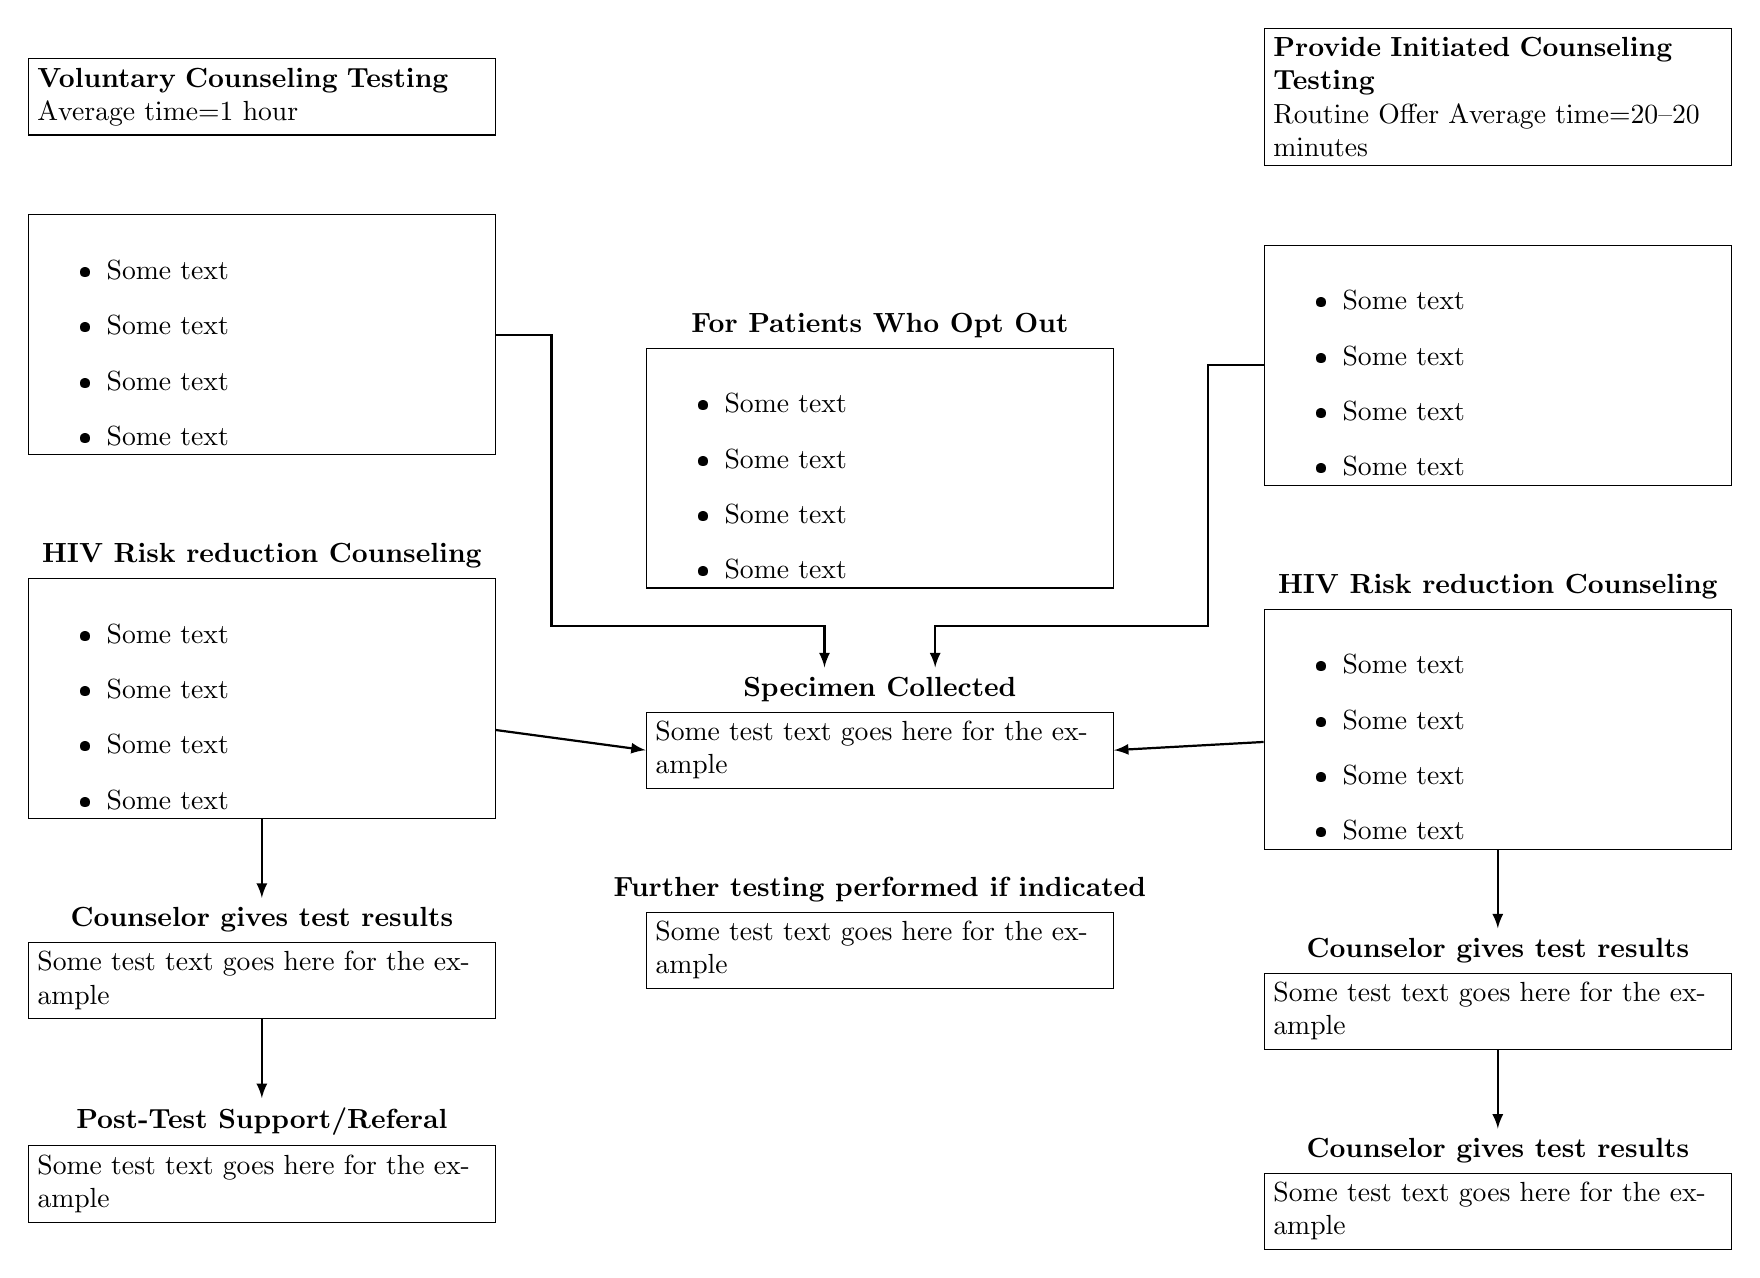
\begin{tikzpicture}[
  mybox/.style={
    draw,
    text width=5.7cm,
    anchor=north
  },
  nobox/.style={
    text width=5.7cm,
    align=center,
    anchor=north,
    font=\bfseries
  },
  arr/.style={
    ->,
    line width=0.8pt
  },
  node distance=1cm and 2cm,
  >=latex
]
% The left part
\node[mybox]
  (left1)
  {\textbf{Voluntary Counseling Testing} \\
  Average time=1 hour
  };
\node[mybox,below=of left1]
  (left2)
  {\begin{itemize}
    \item Some text
    \item Some text
    \item Some text
    \item Some text
   \end{itemize}
  };  
\node[nobox,below=of left2]
  (left3)
  {HIV Risk reduction Counseling};
\node[mybox,below=0pt of left3]
  (left4)
  {\begin{itemize}
    \item Some text
    \item Some text
    \item Some text
    \item Some text
   \end{itemize}
  };  
\node[nobox,below=of left4]
  (left5)
  {Counselor gives test results};
\node[mybox,below=0pt of left5]
  (left6)
  {Some test text goes here for the example};  
\node[nobox,below=of left6]
  (left7)
  {Post-Test Support/Referal};
\node[mybox,below=0pt of left7]
  (left8)
  {Some test text goes here for the example};  

% the middle part
\node[right=of left1,text width=5.5cm] 
  (middle1) {};
\node[nobox,below=2.5cm of middle1]
  (middle2)
  {For Patients Who Opt Out};
\node[mybox,below=0pt of middle2]
  (middle3)
  {\begin{itemize}
    \item Some text
    \item Some text
    \item Some text
    \item Some text
   \end{itemize}
  };  
\node[nobox,below=of middle3]
  (middle4)
  {Specimen Collected};
\node[mybox,below=0pt of middle4]
  (middle5)
  {Some test text goes here for the example};  
\node[nobox,below=of middle5,text width=7cm]
  (middle6)
  {Further testing performed if indicated};
\node[mybox,below=0pt of middle6]
  (middle7)
  {Some test text goes here for the example};  

% the right part     
\node[mybox,right=of middle1]
  (right1)
  {\textbf{Provide Initiated Counseling Testing} \\
  Routine Offer Average time=20--20 minutes
  };
\node[mybox,below=of right1]
  (right2)
  {\begin{itemize}
    \item Some text
    \item Some text
    \item Some text
    \item Some text
   \end{itemize}
  };  
\node[nobox,below=of right2]
  (right3)
  {HIV Risk reduction Counseling};
\node[mybox,below=0pt of right3]
  (right4)
  {\begin{itemize}
    \item Some text
    \item Some text
    \item Some text
    \item Some text
   \end{itemize}
  };  
\node[nobox,below=of right4]
  (right5)
  {Counselor gives test results};
\node[mybox,below=0pt of right5]
  (right6)
  {Some test text goes here for the example};  
\node[nobox,below=of right6]
  (right7)
  {Counselor gives test results};
\node[mybox,below=0pt of right7]
  (right8)
  {Some test text goes here for the example};  

%the arrows  
\path[arr]
  (left4) edge (left5)
  (left6) edge (left7)
  (right4) edge (right5)
  (right6) edge (right7)
  (left4) edge (middle5.west)
  (right4) edge (middle5.east);
\draw[arr]  
  (left2.east) -- 
  ++(20pt,0pt)  |- 
  ([shift={(-20pt,15pt)}]middle4.north) --
  ([shift={(-20pt,0pt)}]middle4.north);
\draw[arr]  
  (right2.west) -- 
  ++(-20pt,0pt)  |- 
  ([shift={(20pt,15pt)}]middle4.north) --
  ([shift={(20pt,0pt)}]middle4.north);

\end{tikzpicture}

\end{document}
